\documentclass{article}
\usepackage[section]{placeins}
\usepackage{graphicx, wrapfig, amsmath, amssymb, physics, hyperref}
\hypersetup{
    colorlinks=true,
    linkcolor=blue,
    filecolor=magenta,      
    urlcolor=cyan,
    }

\author{Yaghoub Shahmari}
\title{Report - Problem Set No 6}
\date{\today}
\graphicspath{ {../Figs/} }

\begin{document}
    \maketitle
    \section*{Problem 1}
    \textbf{Basic description:}

    \textbf{The results:}

    \begin{figure}[!htb]
        \centering
        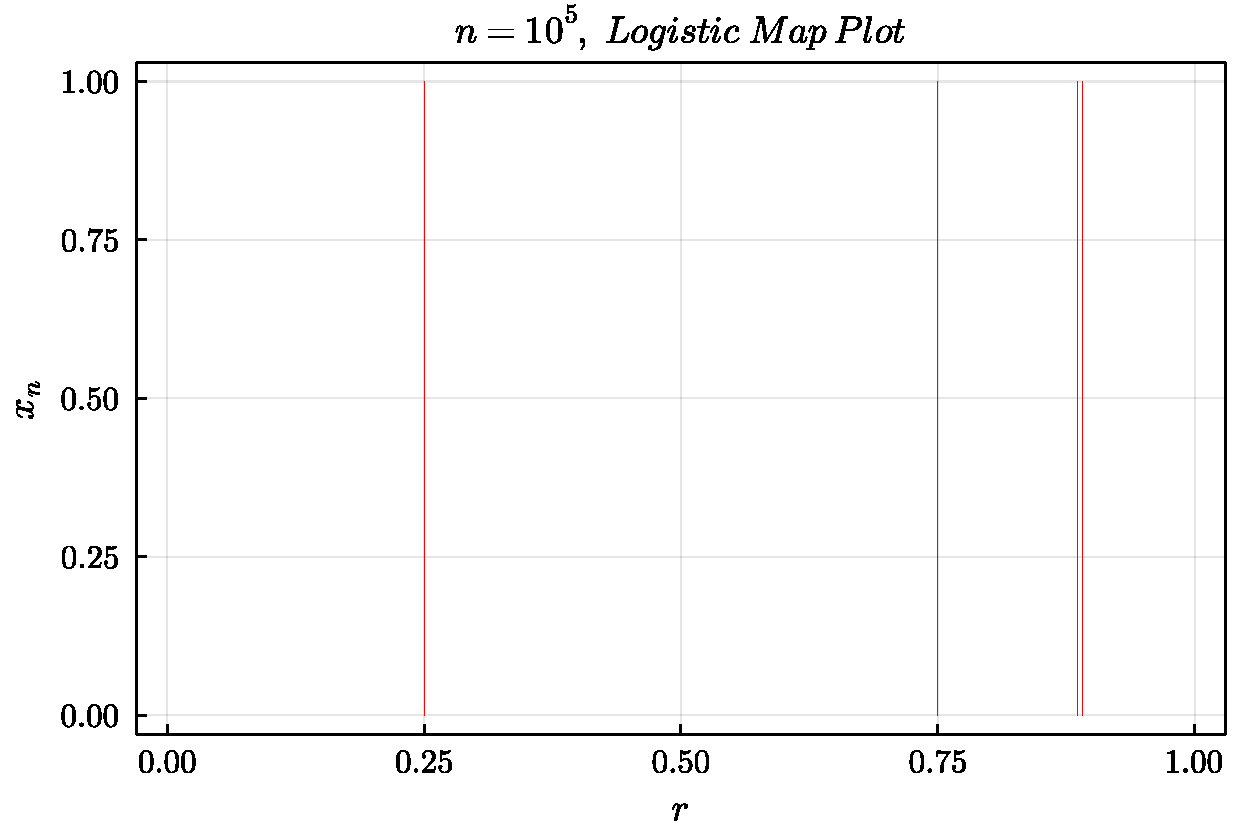
\includegraphics[scale = 0.025]{/Q3/logmap.png}
        \label{fig:1.1}
        \caption{Distribution of answers for both methods.}
    \end{figure}

    \pagebreak

    \centering
    \textbf{The whole data I gathered is in \href{https://github.com/shahmari/ComputationalPhysics-Fall2021/tree/main/ProblemSet7/Data}{this link}}

    Thanks for watching :)
\end{document}